% 2015 年陕西卷（文史类）第 22 题：圆的切线与割线（依固定扫描页重绘，只画拓扑与标号，不按比例）
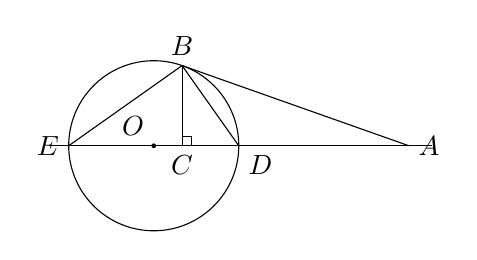
\begin{tikzpicture}[>=stealth,scale=0.72]
  % 圆 O
  \draw (0,0) circle (1.5);
  \fill (0,0) circle (1.2pt);
  \node[above left] at (0,0) {$O$};
  % 割线 A-D-C-O-E
  \draw (-1.85,0)--(4.9,0);
  \coordinate (E) at (-1.5,0);
  \coordinate (C) at (0.5,0);
  \coordinate (D) at (1.5,0);
  \coordinate (A) at (4.5,0);
  \coordinate (B) at (0.5,1.414);
  % 切线与弦
  \draw (B)--(A);
  \draw (B)--(E);
  \draw (B)--(D);
  \draw (B)--(C);
  % 直角标记
  \draw (0.5,0.16)--(0.66,0.16)--(0.66,0);
  % 标号
  \node[above] at (B) {$B$};
  \node[left] at (E) {$E$};
  \node[below] at (C) {$C$};
  \node[below right] at (D) {$D$};
  \node[right] at (A) {$A$};
\end{tikzpicture}
